%%%%%%%%%%%%%%%%%%%%%%%%%%%%%%%%%%%%%%%%%
% The Legrand Orange Book
% LaTeX Template
% Version 2.1.1 (14/2/16)
%
% This template has been downloaded from:
% http://www.LaTeXTemplates.com
%
% Original author:
% Mathias Legrand (legrand.mathias@gmail.com) with modifications by:
% Vel (vel@latextemplates.com)
%
% License:
% CC BY-NC-SA 3.0 (http://creativecommons.org/licenses/by-nc-sa/3.0/)
%
% Compiling this template:
% This template uses biber for its bibliography and makeindex for its index.
% When you first open the template, compile it from the command line with the 
% commands below to make sure your LaTeX distribution is configured correctly:
%
% 1) pdflatex main
% 2) makeindex main.idx -s StyleInd.ist
% 3) biber main
% 4) pdflatex main x 2
%
% After this, when you wish to update the bibliography/index use the appropriate
% command above and make sure to compile with pdflatex several times 
% afterwards to propagate your changes to the document.
%
% This template also uses a number of packages which may need to be
% updated to the newest versions for the template to compile. It is strongly
% recommended you update your LaTeX distribution if you have any
% compilation errors.
%
% Important note:
% Chapter heading images should have a 2:1 width:height ratio,
% e.g. 920px width and 460px height.
%
%%%%%%%%%%%%%%%%%%%%%%%%%%%%%%%%%%%%%%%%%

%----------------------------------------------------------------------------------------
%	PACKAGES AND OTHER DOCUMENT CONFIGURATIONS
%----------------------------------------------------------------------------------------

\documentclass[11pt,fleqn]{book} % Default font size and left-justified equations

\usepackage{ifthen} 
\newboolean{VersionProf}
\setboolean{VersionProf}{false}

\usepackage{wasysym}
\usepackage{esint} % various fancy integral symbols
\usepackage{tikz}
\usepackage{tikz-3dplot}
\usepackage{pgfplots}
\pgfplotsset{compat=1.17}
\usetikzlibrary{patterns}
\usepackage{tkz-euclide} 
\usepackage{mathtools}
\usepackage{xurl}
\usepackage[version=4,arrows=pgf-filled,
textfontname=sffamily,
mathfontname=mathsf]{mhchem}
\usepackage{gensymb}
\usepackage{tabularray}
\usepackage{csquotes}

\usepackage[french]{babel}
\usepackage{dingbat}

\usepackage{environ}
\usepackage{wrapfig}

\NewEnviron{solution}{%
    \ifthenelse{\boolean{VersionProf}}{\begin{solutionA}
        \BODY%*
        \end{solutionA}
    }{%
        \relax%
    }%
}%

\usetikzlibrary {arrows.meta} 

\newcommand{\degC}{{\degree}C}
\newcommand{\dd}{\mathrm{d}}
\newcommand{\div}{\mathrm{div}}
\newcommand{\rot}{\vv{\mathrm{div}}}
\newcommand{\grad}{\vv{\mathrm{grad}}}
\newcommand{\rref}{\mathcal{R}}


\tikzset{
    support/.style={
        pattern=north east lines,
        draw=none,
        minimum width=0.3,
        minimum height=0.6
    }
    ,>=latex
}

\usepackage[d]{esvect}

%SPECIFIC TO THIS CHAPTER
\usepackage{physics}
\usepackage{ifthen}
\usepackage[outline]{contour} % glow around text
\usetikzlibrary{calc} % for pic
\usetikzlibrary{angles,quotes} % for pic
\usetikzlibrary{patterns}
\tikzset{>=latex} % for LaTeX arrow head
\contourlength{1.2pt}

\colorlet{myred}{red!65!black}
\definecolor{myred}{RGB}{55,62,151}
\tikzstyle{ground}=[preaction={fill,top color=black!10,bottom color=black!5,shading angle=20},
                    fill,pattern=north east lines,draw=none,minimum width=0.3,minimum height=0.6]
\tikzstyle{mass}=[line width=0.6,myred,fill=myred!40,rounded corners=1,
                  top color=myred!40,bottom color=myred!20,shading angle=20]
\tikzstyle{rope}=[myred!30,line width=1.2,line cap=round] %very thick

% FORCES SWITCH
\tikzstyle{force}=[->,myred,ultra thick,line cap=round]
\tikzstyle{Fproj}=[force,myred!60]
\newboolean{showforces}
\setboolean{showforces}{true}
%----------------------------------------------------------------------------------------

\input{structure} % Insert the commands.tex file which contains the majority of the structure behind the template

\renewcommand{\topfraction}{0.98}
\renewcommand{\bottomfraction}{0.98}
\renewcommand{\textfraction}{0.02}
\renewcommand{\floatpagefraction}{0.98}

\begin{document}

%----------------------------------------------------------------------------------------
%	TABLE OF CONTENTS
%----------------------------------------------------------------------------------------

%\usechapterimagefalse % If you don't want to include a chapter image, use this to toggle images off - it can be enabled later with \usechapterimagetrue

\chapterimage{cyclone.jpg} % Table of contents heading image

%\pagestyle{empty} % No headers

%\tableofcontents % Print the table of contents itself

%\cleardoublepage % Forces the first chapter to start on an odd page so it's on the right

%\pagestyle{fancy} % Print headers again



%\part{\'{E}lectromagnétisme}

\setcounter{chapter}{20}

\chapter{Dynamique en référentiel non galiléen}

Les lois que nous connaissons en mécanique (principe d'inertie, principe fondamental de la dynamique, théorème du moment cinétique, théorème de l'énergie cinétique) sont valables exclusivement dans des référentiels galiléens. Néanmoins, il est parfois utile d'étudier un mouvement dans un référentiel qui n'est pas galiléen, les lois usuelles de la mécanique ne semblent alors plus vérifées. C'est le cas par exemple dans un véhicule qui démarre, ou bien dans un référentiel en rotation. On observe alors des phénomènes qui peuvent paraître contre-intuitifs.

Dans ce chapitre, nous allons construire une base théorique permettant d'étudier ce type de mouvement, en se ramenant à l'étude du mouvement dans un référentiel galiléen. Nous allons alors montrer que le caractère non galiléen du référentiel peut se traduire par la notion de pseudo-force d'inertie, comme la pseudo-force centrifuge, d'entraînement, ou de Coriolis.

\section{Cinématique des référentiels}

\subsection{Quelques référentiels usuels}

Avant de démarrer, il est utile de définir quelques référentiels usuels et de nous intéresser au mouvement relatif de ces référentiels, et des conditions dans lesquelles on pourra les considérer comme galiléens ou non. Dans la vie courante, les mouvements que nous observons se décrivent bien dans le référentiel terrestre :
\begin{definition}[Référentiel terrestre]
	Le référentiel terrestre est le référentiel lié au sol en un point donné de la surface de la Terre.
\end{definition}

\begin{capex}
	Dans quelles conditions peut-on considérer que le référentiel terrestre est galiléen ? Citer quelques mouvements pour lesquels on peut faire cette approximation. Donner également quelques manifestations du caractère non galiléen du référentiel terrestre.
\end{capex}

Pour pouvoir expliquer certains mouvements dont la durée est relativement longue, nous aurons besoin de définir d'autres référentiels. Nous pouvons définir les référentiels suivants :
\begin{definition}[Référentiel géocentrique]
	Le référentiel géocentrique est le référentiel dont l'origine est le centre de la Terre. Ses axes sont dirigés vers des étoiles lointaines fixes.
\end{definition}
Nous pouvons également définir le référentiel héliocentrique :
\begin{definition}[Référentiel héliocentrique]
	Le référentiel héliocentrique (ou de Copernic) est un référentiel dont l'origine est située au centre de masse du système solaire et dont les axes sont orientés vers des étoiles lointaines fixes.
\end{definition}

\begin{figure}[htbp]
	\centering 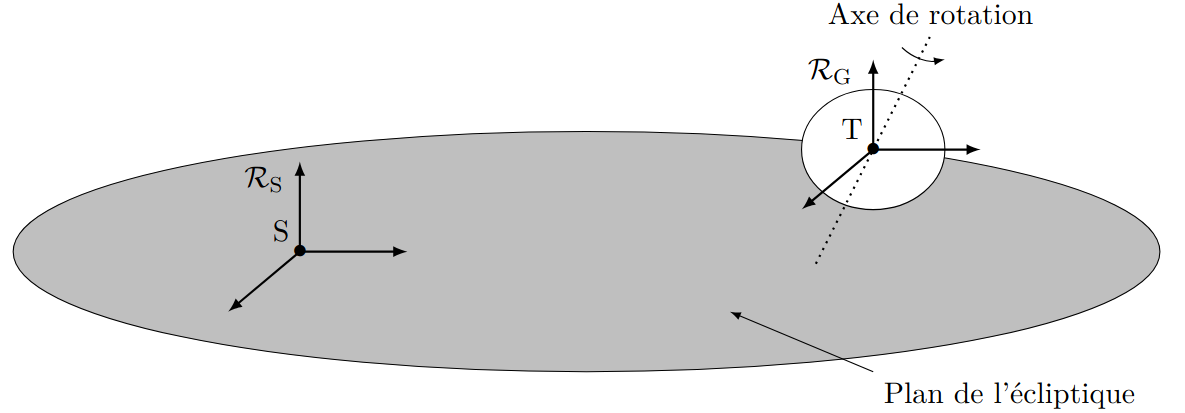
\includegraphics[width=0.71\linewidth]{referentiel_copernic.png} 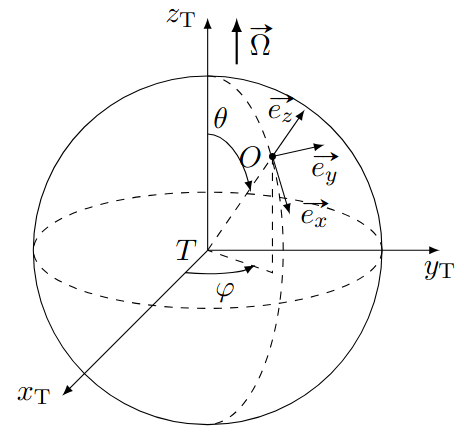
\includegraphics[width=0.28\linewidth]{referentiel_terrestre.png}
	\caption{Référentiels héliocentrique, géocentrique et terrestre. Source : poly de cours de Maxime Champion.}
\end{figure}

Afin de décrire les mouvements des référentiels les uns par rapport aux autres, nous définissons deux types de mouvements :
\begin{definition}[Translation]
	Un référentiel $\rref_2$ est dit en translation par rapport au référentiel $\rref_1$ lorsque le centre $O_2$ de $\rref_2$ se déplace par rapport au centre $O_1$ de $\rref_1$, mais que l'orientation des axes de $\rref_2$ par rapport à $\rref_1$ reste inchangée. 
	On parle de translation rectiligne lorsque le mouvement de $O_2$ est rectiligne dans $\rref_1$, et de translation rectiligne uniforme lorsque ce mouvement est rectiligne uniforme.
\end{definition}

\begin{definition}[Rotation]
	Un référentiel $\rref_2$ est dit en rotation par rapport au référentiel $\rref_1$ lorsqu'il existe un axe $(\Delta)$ de $\rref_2$ immobile dans le référentiel $\rref_1$, et tel que tous les points fixes dans $\rref_2$ ont un mouvement de rotation autour de l'axe $\Delta$ dans $\rref_1$.
	On définit alors le vecteur rotation $\vv \Omega$ colinéaire à $(\Delta)$ dont la norme correspond à la vitesse angulaire de la rotation et le sens est donné par la règle de la main droite.
\end{definition}
\begin{remark}
	Dans ce cours, nous nous limiterons exclusivement aux référentiels en translation et en rotation uniforme autour d'un axe fixe par rapport à un référentiel galiléen.
\end{remark}

\begin{capex}
	Décrire le mouvement du référentiel terrestre par rapport au référentiel géocentrique, ainsi que le mouvement du référentiel géocentrique par rapport au référentiel héliocentrique. Caractériser les propriétés cinématiques de ces mouvements.
\end{capex}

\subsection{Cadre théorique}

Dans tout ce cours, nous nous placerons dans le cadre théorique suivant : nous définissons un référentiel $\rref_1$ supposé galiléen, et nous étudions un mouvement dans un référentiel $\rref_2$ non galiléen, animé d'un mouvement par rapport à $\rref_1$. Ce mouvement est notamment caractérisé par la vitesse du centre $O_2$ de $\rref_2$ par rapport à $\rref_1$, notée $\vv v(O_2/\rref_1)$, et du vecteur rotation $\vv \Omega$ de $\rref_2$ par rapport à $\rref_1$. 

La dérivée d'un vacteur par rapport au temps dépend du référentiel dans lequel cette dérivée est calculée, et nous utiliserons la propriété suivante :
\begin{theorem}[Relation de dérivation composée]
	Soit $\vv u$ un vecteur et $\rref_1$ et $\rref_2$ deux référentiels. On note $\vv \Omega$ le vecteur rotation de $\rref_2$ par rapport à $\rref_1$, alors :
	\begin{equation}
		\left. \frac{\dd \vv u}{\dd t} \right|_{\rref_1} = \left. \frac{\dd \vv u}{\dd t} \right|_{\rref_2} + \vv \Omega \wedge \vv u
	\end{equation}
\end{theorem}


\begin{figure}[htbp]
	\centering 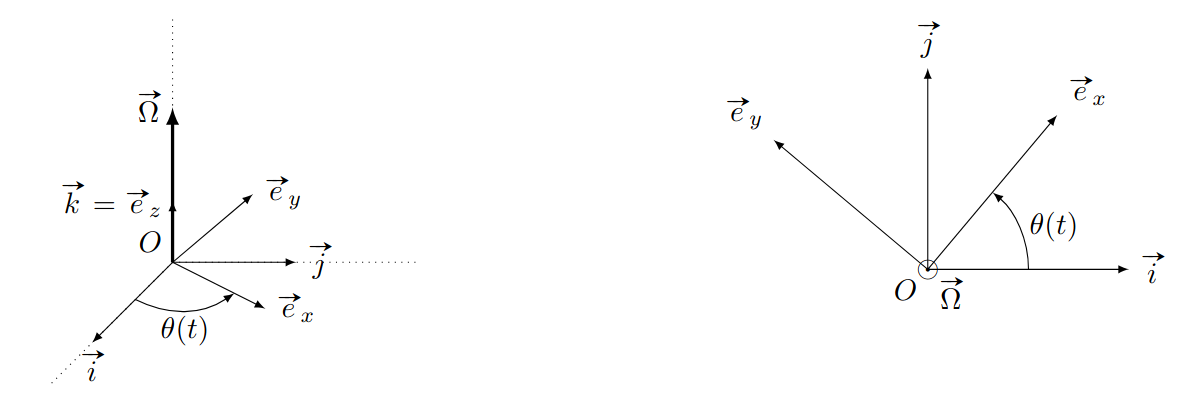
\includegraphics[width=0.75\linewidth]{rotation_reperes.png}
	\caption{Repères associés à deux référentiels en rotation. Source : poly de cours de Maxime Champion.}
\end{figure}

\begin{demonstration}
	Nous choisissons par convention d'orienter l'axe $O_2 z$ du référentiel $\rref_2(O_2,\vv{e_x},\vv{e_y},\vv{e_z})$ parallèlement à l'axe de rotation $(\Delta)$, ainsi on suppose $\vv \Omega = \Omega \vv{e_z}$. Alors nous pouvons écrire :
	\begin{equation}
		\vv u = u_x \vv{e_x} + u_y \vv{e_y} + u_z \vv{e_z}
	\end{equation}
	Dans le référentiel $\rref_2$, les vecteurs de base sont fixes, ainsi :
	\begin{equation}
		\left. \frac{\dd \vv u}{\dd t} \right|_{\rref_2} = \dot u_x \vv{e_x} + \dot u_y \vv{e_y} + \dot u_z \vv{e_z}
	\end{equation}
	En revanche, l'axe de rotation étant orienté selon $(O_2z)$, les vecteurs $\vv{e_x}$ et $\vv{e_y}$ sont mobiles dans le référentiel $\rref_1$ avec :
	\begin{equation}
		\begin{dcases}
			\left. \frac{\dd \vv{e_x}}{\dd t} \right|_{\rref_1} = \Omega \vv{e_y} \\
			\left. \frac{\dd \vv{e_y}}{\dd t} \right|_{\rref_1} = -\Omega \vv{e_x}
		\end{dcases}
	\end{equation}
	Lorsque l'on dérive $\vv u$ par rapport au temps dans $\rref_1$, il faut prendre en compte le fait que ces vecteurs dépendent du temps et :
	\begin{equation}
		\left. \frac{\dd \vv u}{\dd t} \right|_{\rref_1} = \dot u_x \vv{e_x} + \dot u_y \vv{e_y} + \dot u_z \vv{e_z} + u_x \Omega \vv{e_y} - u_y \Omega \vv{e_x}
	\end{equation}
	Nous reconnaissons alors le résultat à démontrer.
\end{demonstration}

\subsection{Composition des vitesses}

Nous pouvons alors déterminer la relation de composition des vitesses. Prenons un point $M$ dont on souhaite étudier le mouvement dans $\rref_2$ qui n'est pas galiléen. Afin d'utiliser les lois de la mécanique, nous avons besoin d'exprimer la vitesse dans le référentiel galiléen $\rref_1$. Pour cela, nous utilisons le fait que :
\begin{equation}
	\vv v(M/\rref_1) = \left. \frac{\dd \vv{O_1M}}{\dd t} \right|_{\rref_1} \quad \mathrm{et} \quad \vv v(M/\rref_2) = \left. \frac{\dd \vv{O_2M}}{\dd t} \right|_{\rref_2}
\end{equation}

\begin{capex}
	Relier la vitesse du point $M$ dans le référentiel $\rref_1$ et dans le référentiel $\rref_2$ à l'aide de la relation de dérivation composée. Ectrire cette vitesse comme une somme de deux termes que l'on interpétera.
\end{capex}

\begin{theorem}[Composition des vitesses]
	Soit $M$ un point matériel, $\rref_1$ et $\rref_2$ deux référentiels en mouvement l'un par rapport à l'autre, et $\vv \Omega$ le vecteur rotation de $\rref_2$ par rapport à $\rref_1$. Alors on peut écrire :
	\begin{equation}
		\vv v(M/\rref_1) = \vv v_{\rm rel} + \vv v_{\rm ent}
	\end{equation}
	où la vitesse relative est la vitesse de $M$ dans le référentiel mobile : $\vv v_{\rm rel} = \vv v(M/\rref_2)$, et la vitesse d'entraînement est la vitesse qu'aurait le point $M$ dans le référentiel $\rref_1$ si $M$ était fixe dans $\rref_2$ : 
	\begin{equation}
		\vv v_{\rm ent} = \vv v(M \in \rref_2/\rref_1) = \vv v(O_2/\rref_1) + \vv{O_2M} \wedge \vv \Omega
	\end{equation}
\end{theorem}

Les vitesses sont ainsi additives : le mouvement du point $M$ peut se décomposer comme la somme du mouvement de $\rref_2$ par rapport à $\rref_1$ au niveau du point $M$, et du mouvement de $M$ dans le référentiel $\rref_2$.

Nous allons désormais dériver une seconde fois afin d'obtenir l'accélération du point $M$ ce qui nous permettra d'appliquer le principe fondamental de la dynamique dans un référentiel galiléen. Nous distinguerons deux cas de translation et de rotation uniforme autour d'un axe fixe.

\section{Dynamique dans un référentiel en translation}

Supposons que notre référentiel est en translation par rapport à un référentiel galiléen. C'est le cas, par exemple, d'une voiture qui freine brusquement (en translation par rapport au référentiel terrestre), ou encore du référentiel géocentrique qui est en translation circulaire autour du référentiel héliocentrique.

Dans ce cas, le vecteur rotation est nul et la loi de composition des vitesses devient :
\begin{equation}
	\vv v(M/\rref_1) = \vv v(O_2/\rref_1) + \vv v(M/\rref_2)
\end{equation}
Nous dérivons cette loi dans le référentiel $\rref_1$ afin d'obtenir l'accélération du point $M$ dans le référentiel $\rref_1$ galiléen :
\begin{align}
	\vv a(M/\rref_1) &= \left. \frac{\dd \vv v(M/\rref_1)}{\dd t}\right|_{\rref_1} \\
	&= \left. \frac{\dd \vv v(O_2/\rref_1)}{\dd t}\right|_{\rref_1} + \left. \frac{\dd \vv v(M/\rref_2)}{\dd t}\right|_{\rref_1} \\
	&= \left. \frac{\dd \vv v(O_2/\rref_1)}{\dd t}\right|_{\rref_1} + \left. \frac{\dd \vv v(M/\rref_2)}{\dd t}\right|_{\rref_2} 
\end{align}
où nous avons utilisé à la dernière ligne la formule de dérivation d'un vecteur avec $\vv \Omega = \vv 0$. Nous reconnaissons dans le terme de gauche, l'accélération du centre du repère $\rref_2$ dans le référientiel galiléen $\rref_1$, que nous appellerons \textit{accélération d'entraînement}. Dans le terme de droite, nous reconnaissons l'accélération du point $M$ dans le référentiel $\rref_2$, que nous appellerons \textit{accélération relative}. Nous obtenons alors la formule de composition des accélérations :
\begin{proposition}[Composition des accélérations dans le cas d'une translation]
	Soit $M$ un point matériel, et $\rref_1$ et $\rref_2$ deux référentiels en translation l'un par rapport à l'autre. On appelle \textit{accélération d'entraînement} $\vv a_{\rm ent}$ l'accélération de l'origine $O_2$ du référentiel $\rref_2$ par rapport à $\rref_1$, et \textit{accélération relative} l'accélération du point $M$ dans le référentiel mobile $\rref_2$.Alors l'accélération totale de $M$ est donnée par :
	\begin{equation}
		\vv a(M/\rref_1) = \vv a_{\rm ent} + \vv a_{\rm rel} = \vv a(O_2/\rref_1) + \vv a(M/\rref_2)
	\end{equation}
\end{proposition}

\begin{capex}
	Montrer que le principe fondamental de la dynamique reste valable dans le référentiel $\rref_2$, à condition d'ajouter une force fictive $\vv f_{\rm ie}$ dont on précisera l'expression.
\end{capex}

Nous en concluons que tout se passe comme si une force fictive supplémentaire agissait sur le mouvement, qui est appelée force d'inertie d'entraînement :
\begin{theorem}[Principe fondamental de la dynamique dans un référentiel en translation]
	Soit $M$ un point matériel de masse $m$, et $\rref_2$ un référentiel mobile en translation par rapport à un référentiel galiléen avec une accélération d'entraînement $\vv a_{\rm ent}$. Alors le principe fondamental de la dynamique reste applicable dans $\rref_2$ à condition d'ajouter une \textit{pseudo-force d'inertie d'entraînement} :
	\begin{equation}
		\vv f_{\rm i.e.} = - m \vv a_{\rm ent}
	\end{equation}
\end{theorem}


\begin{figure}[htbp]
	\centering 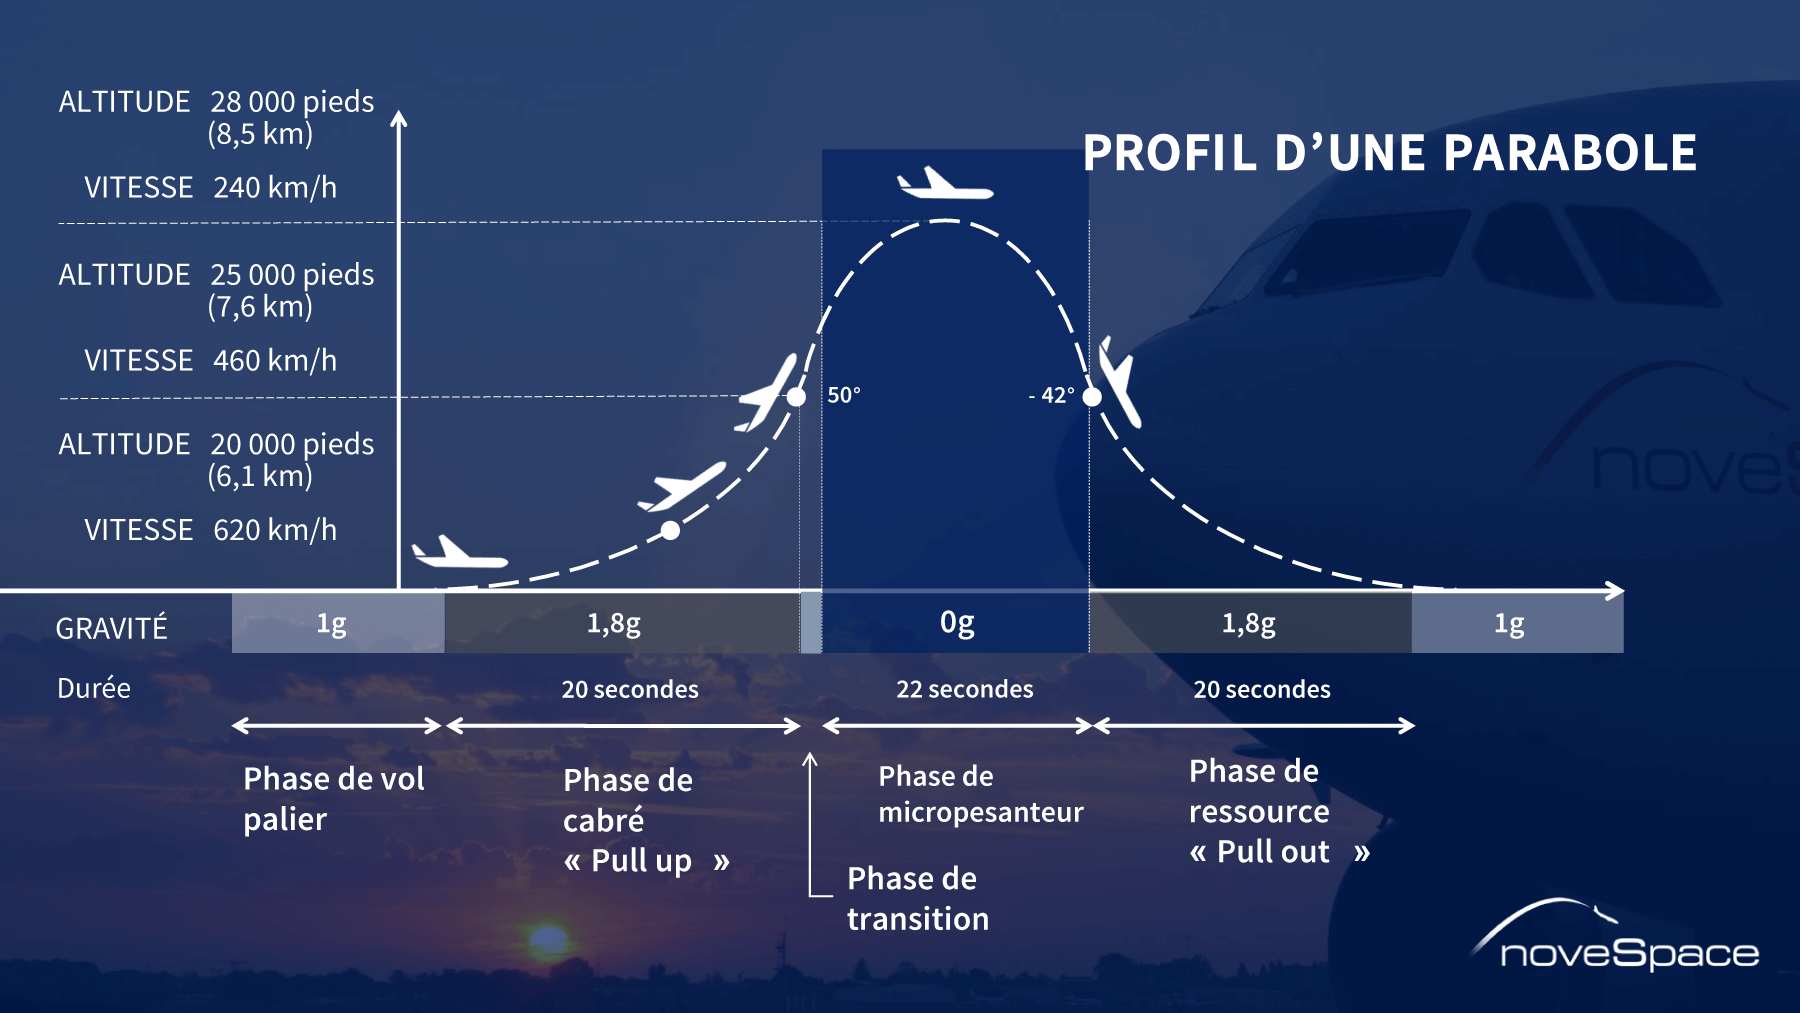
\includegraphics[width=0.8\linewidth]{zerog.png}
	\caption{Schéma d'un vol zéro-$g$. Source : Novespace.}
\end{figure}

\begin{encart}[Les vols zéro-$g$]
	Un nombre important d'expériences scientifiques doivent être réalisées en impesanteur. Cela peut être réalisé dans la station spatiale internationale, ou bien dans des vols paraboliques dits "zéro-$g$". Lors de ces vols, l'avion décrit une trajectoire parabolique telle que l'accélération vertivale de l'appareil soit exactement $\vv a_{\rm ent} = \vv g$. Dans ce cas, dans le référentiel de l'avion, la force d'inertie d'entraînement $\vv f_{\rm i.e.} = - m \vv g$ et le poids $\vv P = m \vv g$ se compensent exactement. La pesanteur n'est alors plus ressentie. 
	
	En automne dernier, par exemple, des étudiants de l'école d'ingénieur Junia à Lille ont réalisé en vol zéro-$g$ une expérience permettant de mesurer la pression de radiation sur une voile solaire miniature.
\end{encart}

\section{Cas de la rotation autour d'un axe fixe}

Nous nous intéressons désormais au cas où le référentiel $\rref_2$ est en rotation par rapport à $\rref_1$ autour d'un axe fixe $(\Delta)$. Comme il n'y a pas de translation entre ces référentiels, il est possible de choisir les origines des deux référentiels confondues sur un point de l'axe $(\Delta)$ , nous avons alors $O_1 = O_2 = O \in (\Delta)$.

\begin{capex}
	Exprimer l'accélération du point $M$ dans le référentiel $\rref_1$ en fonction des propriétés cinématiques de $M$ dans $\rref_2$ et du vecteur rotation $\Omega$.
\end{capex}

Nous obtenons la propriété suivante :
\begin{proposition}[Composition des accélérations dans un référentiel en rotation]
	Soit $M$ un point matériel, $\rref_2$ un référentiel en rotation par rapport à un autre référentiel $\rref_1$ autour d'un axe fixe $(\Delta)$, et $O$ l'origine de ces deux référentiels située sur l'axe $(\Delta)$. On note $\vv r = \vv{OM} = \vv r_\perp + \vv r_\parallel$ la décomposition du vecteur position selon les directions parallèle et perpendiculaire à l'axe de rotation. Alors nous pouvons écrire :
	\begin{equation}
		\vv a(M/\rref_1) = \vv a_{\rm ent} + \vv a_{\rm rel} + \vv a_{\rm cor}
	\end{equation}
	où :
	\begin{itemize}
		\item $\vv a_{\rm ent}$ est l'accélération qu'aurait le point $M$ dans $\rref_1$ s'il était lié à $\rref_2$. Comme le mouvement est une rotation autour d'un axe fixe, il s'agit d'une accélération centripète :
			\begin{equation}
				\vv a_{\rm ent} = - {\vv \Omega}^2 \vv r_{\perp}
			\end{equation}
		\item $\vv a_{\rm rel}$ est l'accélération du point $M$ dans le référentiel mobile :
			\begin{equation}
				\vv a_{\rm rel} = \vv a(M/\rref_2)
			\end{equation}
		\item $\vv a_{\rm cor}$ est l'accélération de Coriolis, liée à la combinaison entre la vitesse de la particule dans le référentiel $\rref_2$ et la rotation de ce dernier :
			\begin{equation}
				\vv a_{\rm cor} = 2 \vv \Omega \wedge \vv v(M/\rref_2) = 2 \vv \Omega \wedge \vv v_{\rm rel}
			\end{equation}
	\end{itemize}
\end{proposition}

Nous pouvons alors conclure quant à l'existence de deux pseudo-forces d'inertie dans le cas d'une rotation autour d'un axe fixe :
\begin{theorem}[Principe fondamental de la dynamique dans un référentiel en rotation]
	Soit $M$ un point matériel de masse $m$, $\rref_2$ un référentiel en rotation par rapport à un référentiel galiléen autour d'un axe fixe à la vitesse angulaire $\Omega$. On se place dans un système de coordonnées cylindriques dont l'axe $(Oz)$ coïncide avec l'axe de rotation. Alors on peut appliquer le principe fondamental de la dynamique dans le référentiel mobile $\rref_2$ en rajoutant deux pseudo-forces d'inertie :
	\begin{itemize}
		\item La pseudo-force d'inertie d'entraînement (communément appelée \textit{force centrifuge}) $\vv f_{\rm i.e.} = m r \Omega^2 \vv{e_r}$
		\item La pseudo-force d'inertie de Coriolis $\vv f_{\rm i.c.} = - 2 m \vv \Omega \wedge \vv v_{\rm rel}$
	\end{itemize}
	où $\vv v_{\rm rel}$ est la vitesse du point $M$ dans le référentiel tournant $\rref_2$.
\end{theorem}

\begin{figure}[htbp]
	\centering 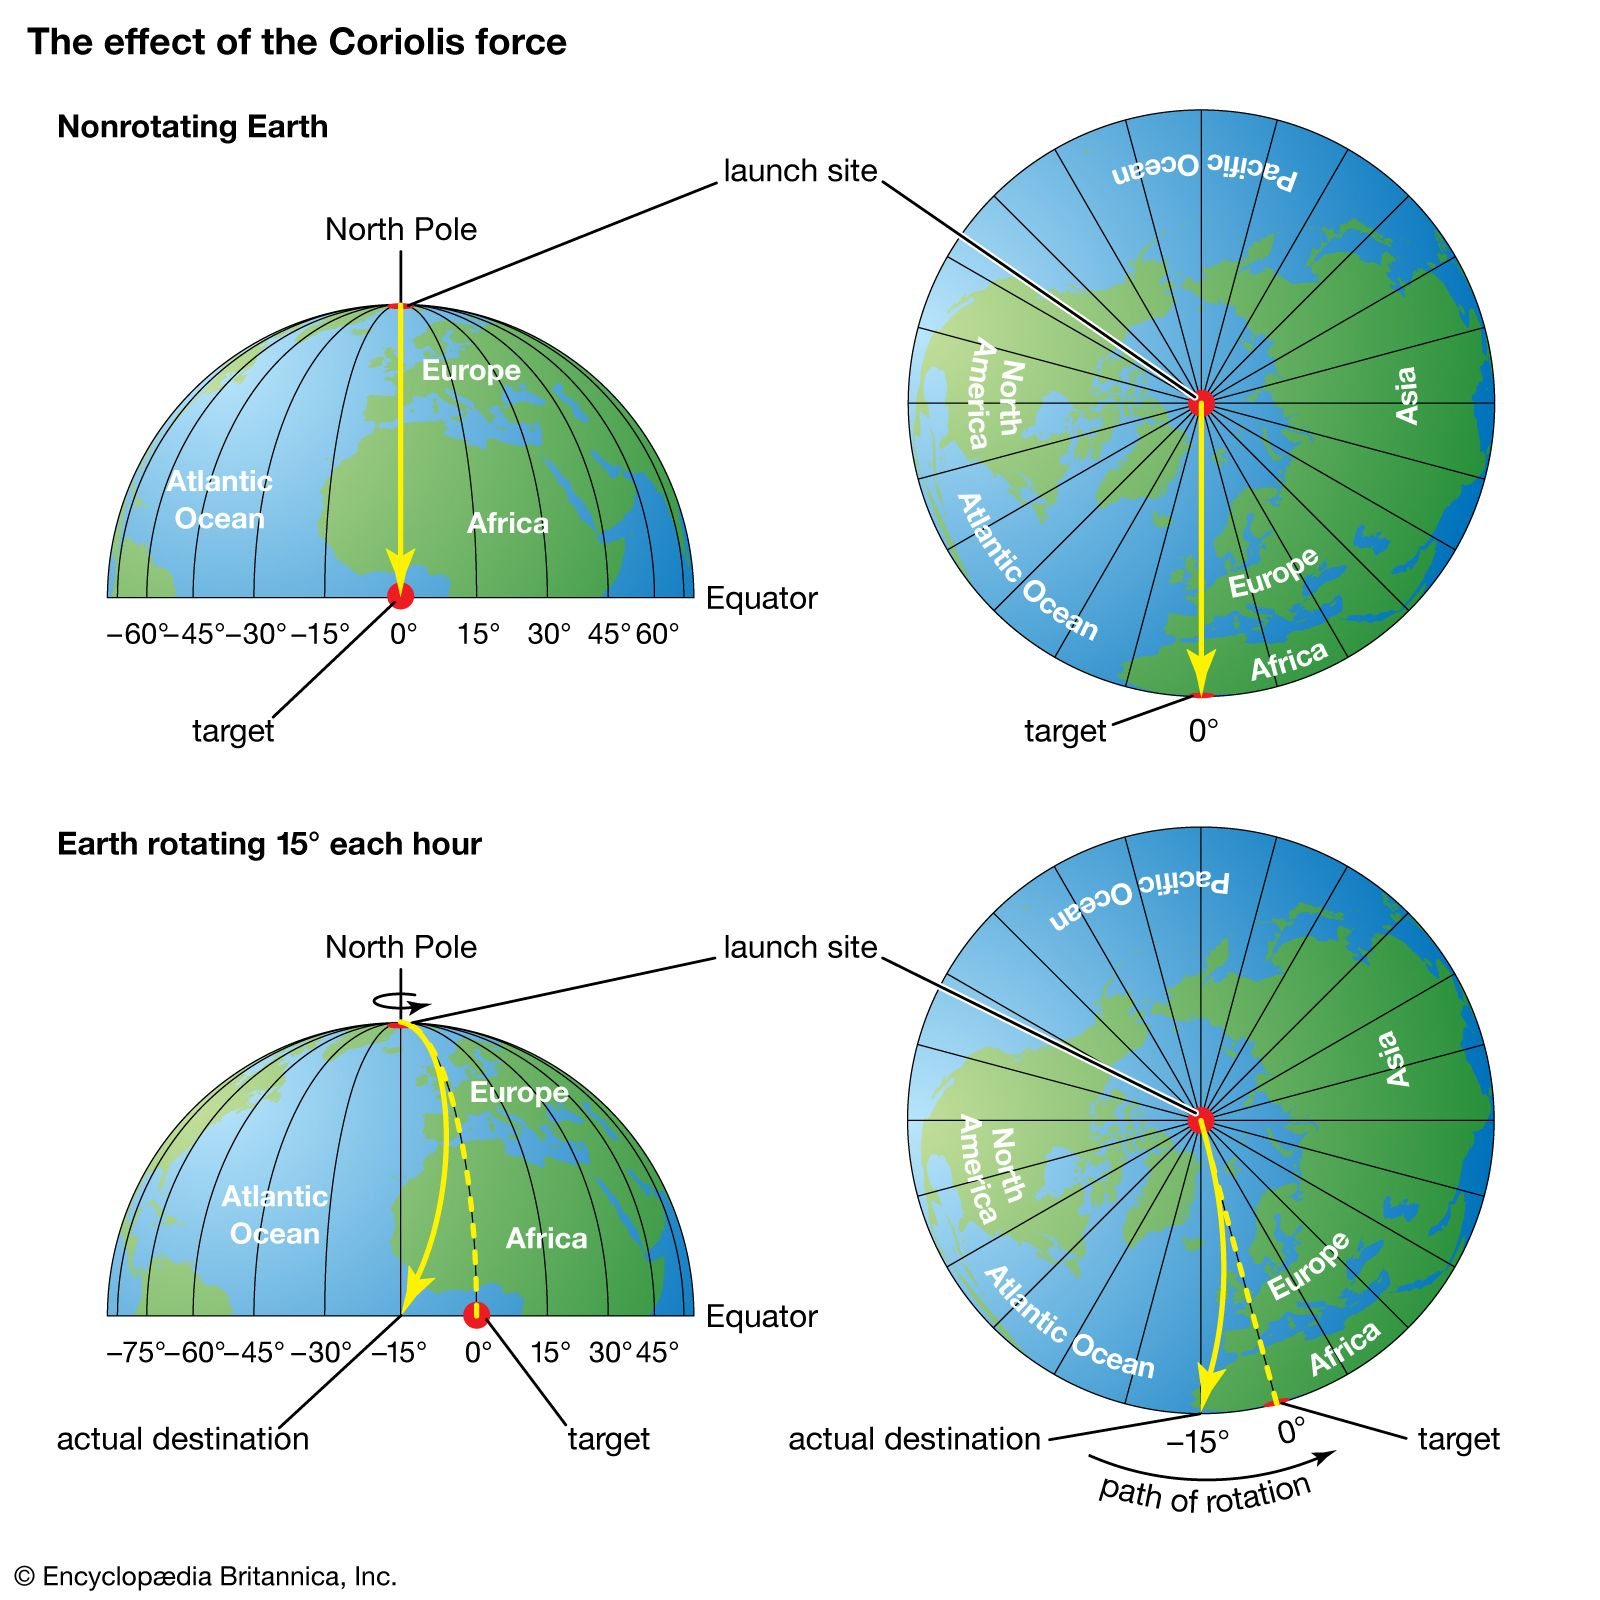
\includegraphics[width=0.75\linewidth]{coriolis.jpg}
	\caption{Schéma explicitant le rôle de la composition des vitesses dans la pesudo-force de Coriolis. Source : Encyclopedia Britannica.}
\end{figure}

\begin{encart}[La forme de la Terre]
	En raison de la pseudo-force d'inertie d'entraînement, la rotation de la Terre cause un léger bombement de la surface, ainsi le rayon de la Terre est plus important à l'équateur qu'au niveau des pôles. Ceci a été découvert lors d'expéditions scientifiques françaises : Bouguer, en se rendant au Pérou, a constaté que la période d'oscillation d'un pendule y était plus longue qu'à Paris. L'explication est double :
	\begin{itemize}
		\item D'une part, en raison de la rotation de la Terre, la pseudo-force d'inertie d'entraînement (centrifuge) est plus forte près de l'équateur et contribue donc à réduire l'effet de l'attraction gravitationnelle de la Terre ;
		\item D'autre part, la Terre étant plus large à l'équateur, on s'y trouve plus éloigné du centre de la Terre ce qui contribue également à une diminution de l'intensité du champ de gravitation.
	\end{itemize}
	Les mesures de Bouguer ont été fortement controversées, si bien qu'il a été décidé de mener deux expéditions scientifiques en parallèle pour mesurer le rayon de courbure de la Terre par triangulation, au pôle Nord et en Amérique latine. Les résultats ont montré sans appel que la Terre était effectivement aplatie aux pôles.
\end{encart}


\begin{figure}[htbp]
	\centering 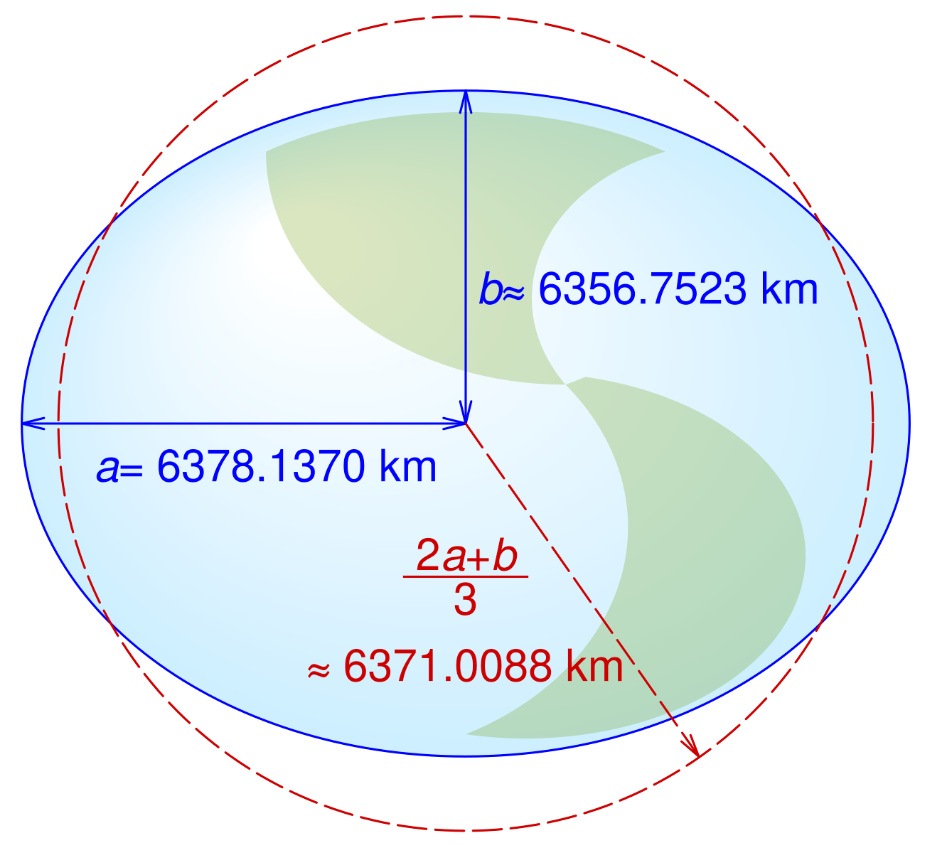
\includegraphics[width=0.5\linewidth]{forme_terre.png}
	\caption{Forme de la Terre. Source : Wikimedia Commons.}
\end{figure}

\begin{encart}[Une manifestation des forces d'inertie : les cyclones tropicaux]
	Les cyclones tropicaux sont associés à des vents puissants qui tournent autour du centre du phénomène. Ceci s'explique par le caractère non galiléen du référentiel terrestre. 

	En effet, la circulation primaire du cyclone est liée au dégagement d'énergie lors de la liquéfaction de la vapeur d'eau (convertie sous forme de pluies) au niveau du centre de la tempête. Ce dégagement d'énergie provoque une élevation de la température, et donc une diminution locale de la densité de l'air. L'air s'élève donc en altitude. Par conservation de la masse, ceci va provoquer une convergence des vents au niveau de la surface. Mais, en raison de la force d'inertie de Coriolis, le vent est dévié vers la droite dans l'hémisphère Nord, et vers la gauche dans l'hémisphère Sud. L'équilibre entre la force de pression (qui puisse l'air au centre du cyclone) et la force d'inertie de Coriolis (qui le dévie vers la droite) implique que le vent tourne dans le sens trigonométrique dans l'hémisphère Nord et dans le sens horaire dans l'hémisphère Sud. 

	Cet équilibre entre les deux forces implique que le cyclone réalise un tour sur lui-même en environ une journée. Sachant que la vitesse des vents à grande distance est de l'ordre de 100\,km/h, on en déduit que le périmètre du cyclone est d'environ 2400\,km, soit un diamètre de l'ordre de 800\,km. Plus la latitude est élevée, plus la force de Coriolis est intense, et plus le cyclone est petit : on observe ainsi un rétrécissement des cyclones lorsqu'ils se déplacent de la Caraïbe vers le golfe du Mexique et les Etats-Unis.

	Par conservation du moment cinétique, lorsque l'air se rapproche du centre du cyclone, sa vitesse orthoradiale ne cesse d'augmenter et les vitesses atteintes deviennent très importantes, ce qui explique les vents violents observés au niveau des cyclones. Dans cette région, le vent fait un tour sur lui-même très rapidement si bien que l'on peut considérer le référentiel terrestre comme galiléen. Néanmoins, dans le référentiel lié au cyclone (en rotation par rapport au référentiel terrestre), les vitesses très importantes sont à l'origine d'une force d'inertie d'entraînement non négligeable qui empêche l'air de pénétrer au centre du cyclone, on a ainsi la formation d'un oeil au centre de la structure et le vent continue à tourner autour de l'oeil.
\end{encart}

\begin{capex}
	On s'intéresse aux phénomènes suivants : un cyclone (taille de 1000\,km, vent de 100\,km/h), l'oeil d'un cyclone (taille de 10\,km, vent de 300\,km/h), une tornade (quelques dizaines de mètres, vent de 100\,km/h), un tourbillon océanique (taille de 50\,km, courants de l'ordre de 10\,cm/s), un tourbillon dans un lavabo. Dans chacun de ces cas, dire si le caractère non galiléen du référentiel terrestre joue un rôle important. Comparer la pseudo-force d'inertie de Coriolis à la pseudo-force d'inertie d'entraînement.
\end{capex}

\begin{figure}[htbp]
	\centering 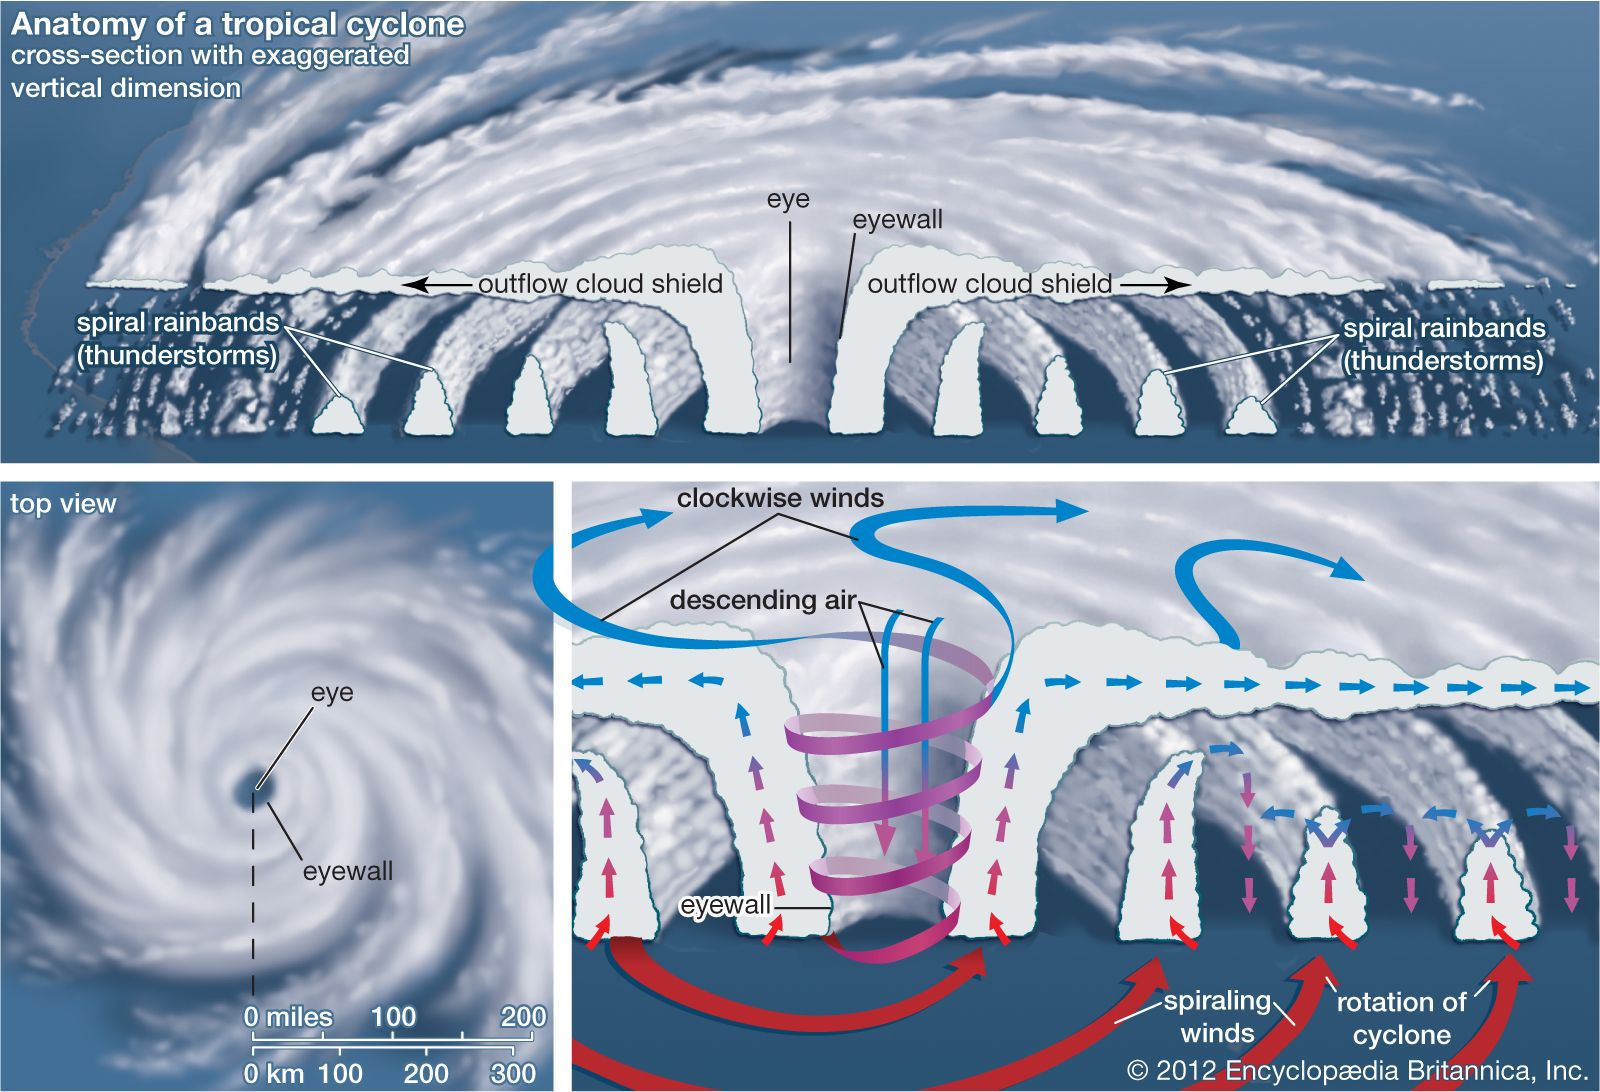
\includegraphics[width=\linewidth]{cyclone_schema.jpg} 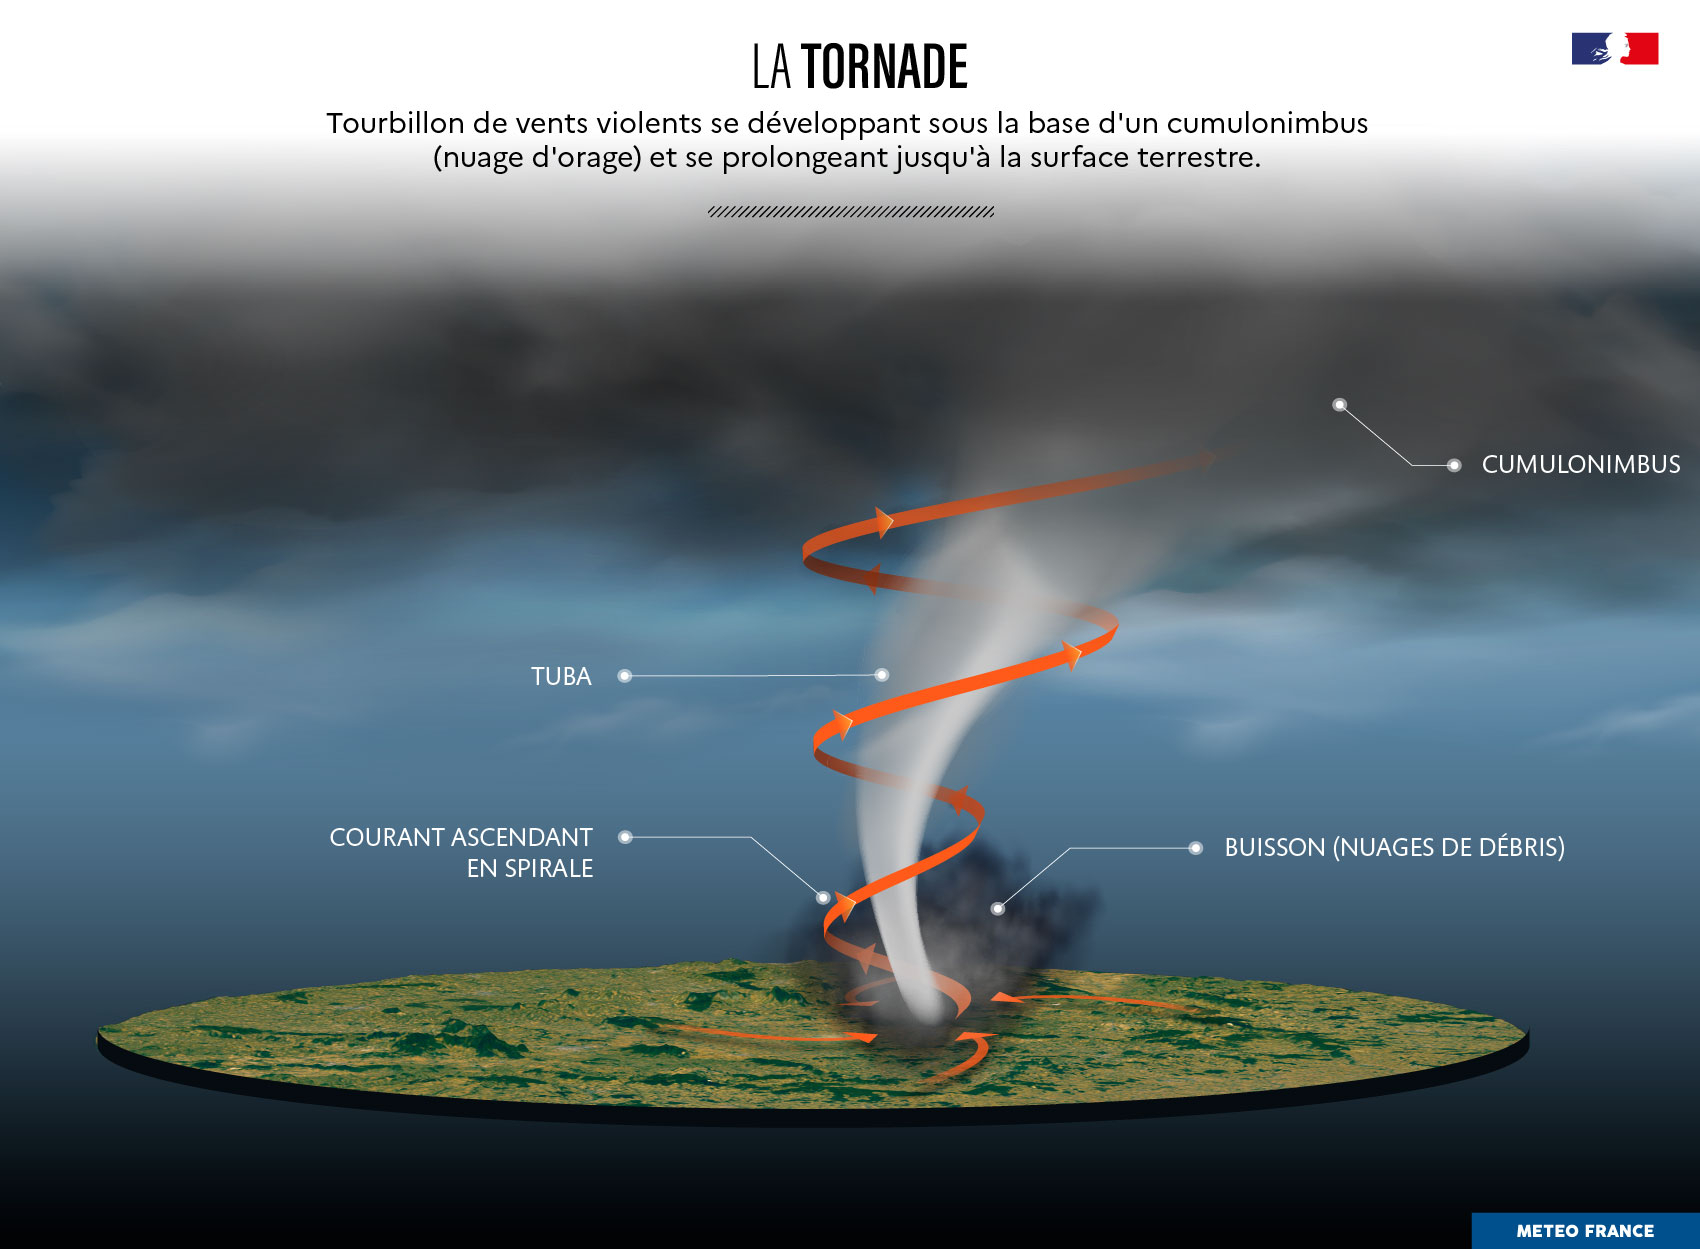
\includegraphics[width=0.7\linewidth]{tornade.jpg}
	\caption{Schémas d'un cyclone et d'une tornade. Sources : Météo-France, UK Royal Meteorological Society.}
\end{figure}
\end{document}
